\section{Motivation and Background}
\todo[inline]{Assuming Introduction has a sentence or two about the
programmability problem.}


Heterogeneity of hardware resources has led to a diverse landscape
of different programming models, run-time systems, profiling and debugging tools
for application development. The differences are so deep that programmers are
often experts on only one class of device, e.g., an expert GPU programmer will
not have much DSP expertise and vice-versa. This is highly inefficient and
unproductive: we cannot expect applications to use a separate language for each
class of compute unit. If we want applications to use the full range of
available hardware to maximize performance or energy efficiency or both, the
programming environment has to provide common abstractions for available
hardware compute units.

OpenCL and RenderScript have been proposed to solve this problem. They are
designed to accelerate data parallel computation intensive part of application
code by allowing workload to be executed on multiple processing cores, GPUs,
DSPs or a combination of these. Here we give a brief overview of OpenCL and
RenderScript.


\subsection{OpenCL}
OpenCL was initiated by Apple Inc. and is managed by the Khronos
Group~\cite{Khronos:url}. It allows the application developers to write
data parallel computation intensive parts of their application for an abstract
hardware model, without using low level hardware specific function calls.

An OpenCL application is composed of two parts: an OpenCL host program and a
set of one or more kernels. The kernels, written in restricted C99 syntax,
specify functions that are to be executed in data parallel fashion. The OpenCL
host program identifies the device on which the OpenCL kernel would be
executed, sets up the environment, allocate memory on the device, copy data
into the device memory and enqueue the kernel execution on the device.

In the Android world, where all application execute on Dalvik virtual machine,
an application using OpenCL has a third component as well. This is the Java
host code which would initialize the application, read in the inputs and use
JNI calls to invoke OpenCL host code.

OpenCL is designed to be portable across a wide range of devices. However,
developers often use hardware specific parameters such as the size of OpenCL
work-group, shared memory size to obtain better performance on specific
hardware. This harms the portability of OpenCL application kernel code.



\subsection{RenderScript}
RenderScript was released by Google as an official computing framework in
2011~\cite{RenderScript}. The motivation behind is to provide
performance and portability across SoC architectures for Android devices.

A RenderScript application consists of three parts: (1) Java application host
code written by the developer that runs on Dalvik VM, (2) RenderScript code
written in restricted C99 syntax containing one or more kernels, and (3)
auto-generated Java code that helps the application host code to communicate with
the RenderScript kernel code, allowing functions such as memory binding between the
host program and the kernels.

\begin{figure}
\centering
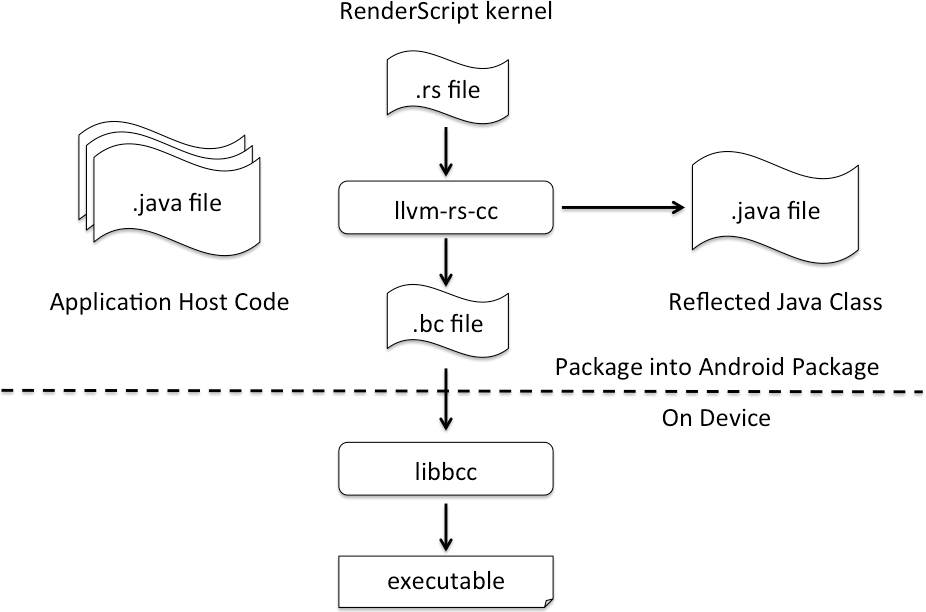
\includegraphics[scale=0.28]{figs/renderscript-compile.png}
\caption{RenderScript Compilation Flow}
\label{fig:RSCompilation}
\centering
\end{figure}

RenderScript compilation flow is shown in Figure~\ref{fig:RSCompilation}.
First, \fix{llvm-rs-cc} utility is used to compile RenderScript kernels to
LLVM~\cite{LLVM:CGO04} bitcode files. The LLVM IR provide support for a wide range of hardware
devices including CPUs, GPUs and DSPs. 
As part of the RenderScript compilation step, corresponding reflected Java classes
are generated via the  the \fix{llvm-rs-cc} tool.
Then after, the application host code, the reflected Java classes and bitcode
are bundled together into the Android application package (\fix{*.apk} file).
During execution, the RenderScript
runtime invokes \fix{libbcc}, the RenderScript back-end compiler, to translate
bitcode into appropriate machine code.



